%\documentclass[10pt]{beamer}
\documentclass[xcolor={dvipsnames}]{beamer}

\usetheme{CambridgeUS}
\usepackage{multirow}

\definecolor{redUnipd}{HTML}{9b0014}
\definecolor{grayUnipd}{HTML}{444F51}
\definecolor{myblue}{HTML}{317a9b}
%\definecolor{Black}{RGB}{0,62,114}
\newcommand{\bbf}[1]{\textcolor{black}{\bf #1}}
\newcommand{\rbf}[1]{\textcolor{redUnipd}{ #1}}
\usefonttheme{structurebold}
%\usecolortheme[named=myblue]{structure}
\setbeamercolor*{structure}{bg=white,fg=redUnipd}
\setbeamercolor{frametitle}{bg=white,fg=redUnipd}
\setbeamercolor{titlelike}{bg=white,fg=redUnipd}
\setbeamercolor*{palette primary}{use=structure,fg=redUnipd,bg=white}
\setbeamertemplate{navigation symbols}{}
\setbeamertemplate{title page}[default][colsep=-4bp,rounded=true]
%\setbeamertemplate{itemize items}{$\circ$}
\setbeamertemplate{enumerate items}[default]
\setbeamertemplate{section in toc}[sections numbered]
\setbeamertemplate{subsection in toc}[subsections numbered]
\setbeamertemplate{itemize items}[square]
%\textopenbullet
%\usepackage{marvosym}
%\setbeamertemplate{itemize items}{$\Neutral$}

\usepackage{pgfpages}
%\pgfpagesuselayout{resize to}[a4paper, 
%                                border shrink=1.5cm,
%                                landscape]


\usepackage[T1]{fontenc}
%
\usepackage[english]{babel}
\usepackage{graphicx}
\usepackage{booktabs}
\usepackage{latexsym}
\usepackage{subfigure}
\usefonttheme{professionalfonts}
%\usepackage{enumitem}
\usepackage{amsmath,amssymb}
\usepackage[latin1]{inputenc}
%\setbeamercovered{dynamic}
\usepackage{Sweave}
\usepackage[english]{babel}
\usepackage{tikz,comment,amssymb}
\usetikzlibrary{shapes}
\setbeamertemplate{blocks}[rounded][shadow=false]

\newcommand{\bb}[1]{\begin{block}{#1}}
\newcommand{\eb}{\end{block}}
\newcommand{\bi}{\begin {itemize}}
\newcommand{\ei}{\end{itemize}}
\newcommand{\be}{\begin {enumerate}}
\newcommand{\ee}{\end{enumerate}}
\linespread{1.05}

\newcommand{\bfr}[1]{\begin{frame} \frametitle{#1}}

\AtBeginSection[] {
  \begin{frame}<beamer>
    \frametitle{Outline}
    \tableofcontents[currentsection]
  \end{frame}
}


\title[]{The Labyrinth of Multiple Testing: how to avoid the pitfall of false positives \\
\vspace*{1cm} \large FDR control}
\subtitle{\vspace*{2cm} \small 12th SISMEC National Congress 2023}
\date{}
\author[\hspace{5cm}]{Livio Finos and Angela Andreella}
%\logo{
\includegraphics[scale=.05]{figures/logoUnipd.jpg}}

\begin{document}

\begin{frame}
  \titlepage
\end{frame}
% Goeman, A Solari

%%%%%%%%%%%%%%%%%%%%%
\begin{frame}
I thank Aldo Solari, Jelle Goeman and Florian Klinglmueller for the ideas and the materials we shared along these years. The material is the result of all this resoning together.

\end{frame}

\section{False Discovery Rate (FDR)}
\subsection{Definition}

% \begin{center}
% \begin{tabular}{ l | c c | r }
%                 & \# Non Rifiutate & \# Rifiutate  & Totale\\
% \hline
%   \# $H_0$ & $A_0$ & \rbf{$R_0$} & $m_0$\\
%   \# $H_1$ & $A_1$ & $R_1$ & $m_1$ \\
% \hline
%     & $A$ & \rbf{$R$} & $m$\\
% \end{tabular}
% \end{center}
% \bigskip
% 
% Controllare il \bbf{False Discovery Rate (FDR)}\\ significa definire una procedura che controlli il valore atteso del rapporto dei falsi rifiuti:\\
% $$E( \frac{\#  Falsi\ Rifiuti}{\# Rifiuti} ) =E(\rbf{\frac{R_0}{R}} ) \leq q$$ 
% \bigskip
% solitamente $q=.05$ (analogo $\alpha$)
% \end{frame}

\bfr{A contingency table}

\begin{table}[]
\centering
\begin{tabular}{@{}ll|cc@{}|l}
&              & \multicolumn{2}{c|}{\textbf{Null hypothesis}}  &   \\ 
& \textbf{}    & \multicolumn{1}{c}{\begin{tabular}[c]{@{}c@{}}False\end{tabular}} & \multicolumn{1}{c}{\begin{tabular}[c]{@{}c@{}}True\end{tabular}} &  \multicolumn{1}{|l}{Tot}\\ 
\midrule
\multicolumn{1}{c}{}                       & Rejected     & \multicolumn{1}{l}{{\color[HTML]{3166FF} $S$}}                                     & {\color[HTML]{9A0000} $V$}  &  {\color[HTML]{16c155} $R$}\\
\multicolumn{1}{c}{\multirow{-2}{*}{Test}} & Not rejected & \multicolumn{1}{l}{{\color[HTML]{9A0000} $T$}}                                      & {\color[HTML]{3531FF} $U$}     &   $m -$ {\color[HTML]{16c155} $R$}  \\    \midrule
\multicolumn{1}{c}{}                       & Tot     & \multicolumn{1}{l}{$m_1$}                                     & $m_0$  &  $m$ \\
\end{tabular}
\end{table}

\vspace{1cm}

\rbf{\textbf{False Discovery Proportion}}: \[
\mathrm{FDP} = \left\{ \begin{array}{ll} {\color[HTML]{9A0000} V} /{\color[HTML]{16c155} R} & \textrm{if ${\color[HTML]{16c155} R} > 0$} \\ 0 & \textrm{otherwise}, \end{array} \right.
\]
Defined for every rejected set ${\color[HTML]{16c155} \mathcal{R}} = \# {\color[HTML]{16c155} R}$.

\end{frame}


\bfr{FWER and FDR}

  \bb{Familywise error rate}
   \[ \mathrm{FWER} = \mathbb{P}({\color[HTML]{9A0000} V} > 0) \]
   A procedure controls it if $\text{FWER} \le \alpha$.
   
   FWER focuses on the probability that the rejected set contains any error.
  \eb
  \bb{False discovery rate}
    \[ \mathrm{FDR} = \mathbb{E}(\mathrm{FDP}) \]
    A procedure controls it if $\text{FDR} \le \alpha$
    
    FDR looks at the expected proportion of errors among the rejections.
  \eb
\end{frame}



\subsection{Methods}

\bfr{Benjamini and Hochberg (BH) procedure
\footnote{Benjamini, Y., & Hochberg, Y. (1995). Controlling the false discovery rate: a practical and powerful approach to multiple testing. Journal of the Royal statistical society: series B (Methodological), 57(1), 289-300.}}

    \be
      \item Sort the $p$-values: $p_{(1)}, \ldots, p_{(m)}$
      \item Find $j'$, the largest $j$ such that
      \begin{equation*}
          p_{(j)} \leq j\alpha/m = c_j^{BH}
      \end{equation*}
      \item Reject all hypotheses with $p$-values at most $p_{j'}$
    \ee
\end{frame}

\bfr{Benjamini and Hochberg (BH) procedure}
\begin{figure}
    \centering
    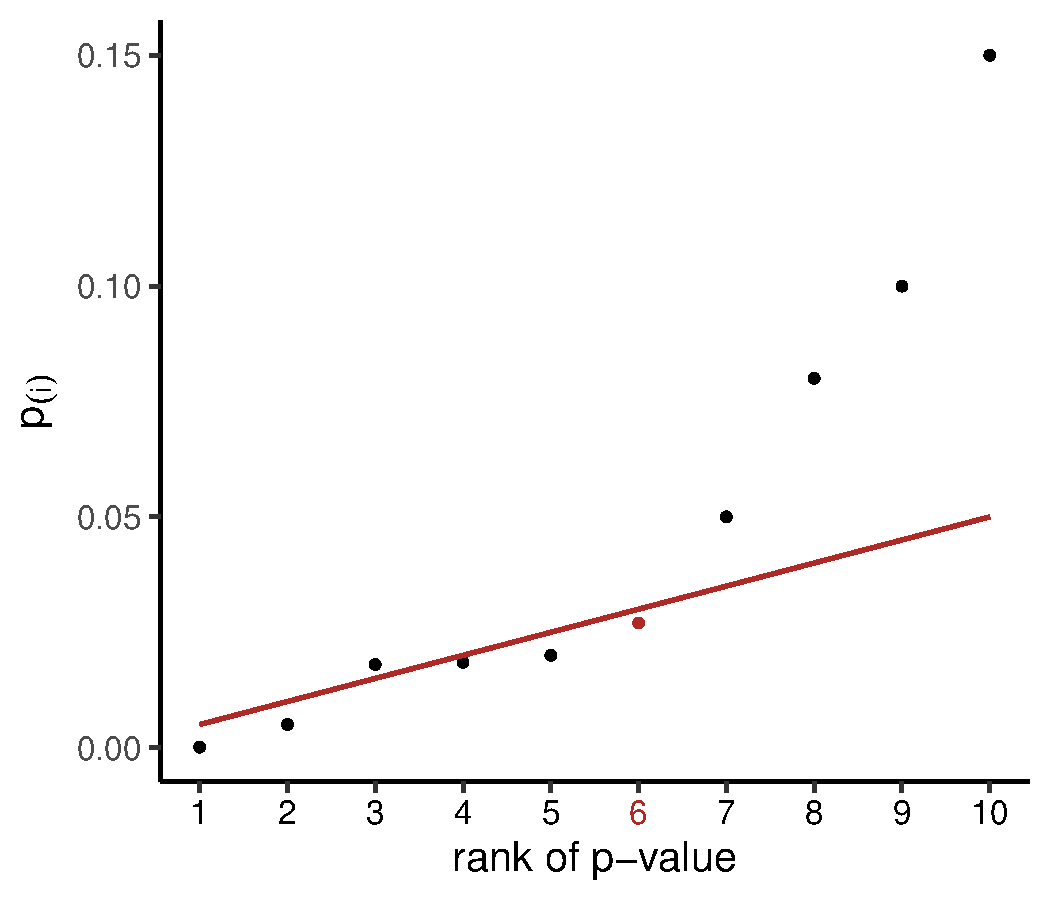
\includegraphics[width = .8\textwidth]{Slides/MTP/plaatjes/bh.pdf}
\end{figure}
\end{frame}

\begin{frame}
\frametitle{Benjamini and Hochberg (BH) procedure}

In this procedure 

\begin{itemize}
    \item FDR control is at $\pi_0\alpha$ (compare Bonferroni), with $\pi_0=m_0/m$
    \vspace{.2cm}
    \item controls FDR is valid under \textbf{independence} and \textbf{positive dependence through stochastic ordering} (i.e.,  non-negatively associated $p$-values):
  \begin{itemize}
      \item \rbf{One-sided tests}: as long as test statistics not negatively correlated
      \item \rbf{Two-sided tests}: If test statistics are (asymptotically) normal
  \end{itemize}
  \vspace{.2cm}
  \item we gain in power with respect to FWER-based methods when $m_0$ is large
  \vspace{.2cm}
  \item $p_{i}^{\text{adjust}} = \dfrac{p_{i}^{\text{raw}} m}{i}$
\end{itemize}
    
\end{frame}


\bfr{Benjamini \&\ Yekutieli (BY)\footnote{Benjamini, Y., \& Yekutieli, D. (2001). The control of the false discovery rate in multiple testing under dependency. Annals of statistics, 1165-1188.}}
Variant of BH valid for any distribution of $p$-values
  \bb{How does it work?}
Same as BH but 
\begin{equation*}
    p_{(j)} \le \dfrac{j \alpha}{m L} = c_j^{BY}
\end{equation*}
where $L=\sum_{j=1}^{m} 1/j$  (es $m=3$: $L= 1/1+1/2+1/3$ )
  \eb
  \bb{In practice}
    \bi
      \item Quite conservative (especially if $m_0$ is large): 
      \begin{itemize}
          \item $c_j^{BY} < c_j^{BH}$
          \item $p_{i}^{\text{adjust}} = \dfrac{p_{i}^{\text{raw}}L m}{i}$
      \end{itemize}
      \item Not often needed, not often used
    \ei
  \eb


\end{frame}

\begin{frame}
\frametitle{Benjamini \&\ Yekutieli (BY)}
    \begin{figure}
    \centering
    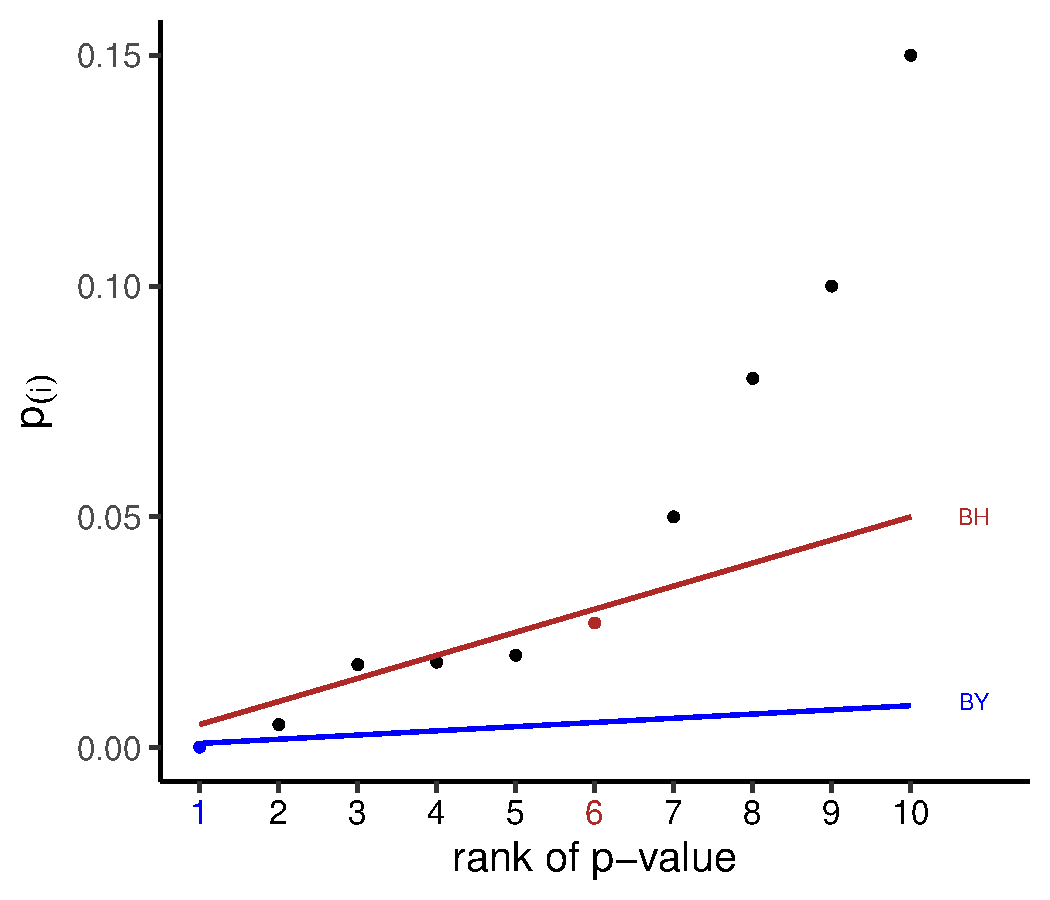
\includegraphics[width = .8\textwidth]{Slides/MTP/plaatjes/BH_BY.pdf}
\end{figure}
\end{frame}

\begin{frame}
\frametitle{False Discovery Rate Control}

BH and BY methods are implemented in \texttt{R} by \texttt{p.adjust}:
\vspace{.3cm}

\begin{itemize}
    \item \texttt{p.adjust(p, "BH")}
    \vspace{.2cm}
    \item \texttt{p.adjust(p, "BY")}
\end{itemize}
    
\end{frame}


\section{FDP estimation}

\begin{frame}
\frametitle{FDP estimation}
\rbf{Difference between FDR control and FDP estimation}
\begin{itemize}
    \item \textbf{FDR control}: starts with the choice of $\alpha$ to be controlled and the procedure finds ${\color[HTML]{16c155} \mathcal{R}}$
    \item \textbf{FDP estimation}: starts with ${\color[HTML]{16c155} \mathcal{R}}$ (not necessarily the hypotheses with top p-values) and finds an estimate (or confidence interval) for FDP of that set.  
\end{itemize}
\vspace{.3cm}

To formulate the point estimation approach:
\begin{itemize}
    \item ${\color[HTML]{9A0000} V}(t) = \# \{ \text{true null } H_i: p_i \le t\}$
    \item $ {\color[HTML]{16c155} \mathcal{R}}(t) =\{H_i: p_i \leq t\}$
\end{itemize}
\vspace{.2cm}

$\rightarrow$ $FDR(t) = \mathbb{E}({\color[HTML]{9A0000} V}(t) / \#{\color[HTML]{16c155} \mathcal{R}}(t))$   with $t \in (0, 1]$

\end{frame}


\bfr{Storey's FDP estimate}

  \bb{Intuition}
    By uniformity of $p$-values under the null 
    \begin{equation*}
        \mathrm{FDP}(t) = {\color[HTML]{9A0000} V}(t) / {\color[HTML]{16c155} R}(t) \approx m_0t/ {\color[HTML]{16c155} R}(t)
    \end{equation*}
  \eb
  \bb{Estimate of $m_0$ (again by uniformity)}
  \[ \hat{m}_0 = \frac{ \#\{p_i > \lambda\}+1}{1-\lambda} \]
  where $0 < \lambda < 1$ constant (e.g., $\lambda = 1/2$, $\lambda = \alpha$).
  \eb
  \bb{Resulting estimate of FDP}
\[    \hat{\mathrm{FDP}}(t)\ =\ \frac{\hat{m}_0t}{{\color[HTML]{16c155} R}(t)}\ =\ \frac{t}{1-\lambda}\frac{\#\{p_i > \lambda\}+1}{\#\{p_i \leq t\}} \]
  \eb
\end{frame}


%\bfr{Storey's FDP estimate}
%  \begin{tikzpicture}[scale=.7]
%    \draw[help lines, ->] (0,0)--(10,0);
%    \draw[help lines, ->] (0,0)--(0,8) ;
%    \path(0,8) node[left] {1};
%    \path(0,0) node[left] {0};
%    \path(10,0) node[below] {$m$};
%    \path(0,0) node[below] {1};
%    \draw plot[smooth, very thick] coordinates{(0,0) (1,0.0024) (2,.036) (3,.152) (4,.448) (5,.948) (6,1.74) (7,2.98) (8,4.47) (9,6.17) (10,8)};
%    \draw (-.1,4) node[left] {$\lambda$} -- (0.1,4);
%    \draw[fill] (7.73,4) circle(2pt);
%    \draw[fill] (10,8) circle(2pt);
%    \draw[help lines, ->] (10,8) -- (5.48,0);
%    \draw[help lines] (0,4) -- (7.73,4);
%    \draw (5.48, .1) -- (5.48, -.1);
%    \path (2.79, -.5) node {$m-\hat{m}_0$};
%    \path (7.74, -.5) node {$\hat{m}_0$};
%    \path (-1,4) node[rotate=90] {$p$-value};
%    \path (5,-1) node {rank of $p$-value};
%    \end{tikzpicture}
%\end{frame}


\bfr{Storey's FDP estimate}

Storey's estimate is sometimes used as a way to control FDR, rather than as a way to estimate FDP: selecting the highest value of $t$ such that the estimate $\hat{\text{FDP}} \le \alpha$.

  \bb{Close relationship with BH}
    Alternative way of constructing BH rejected set
    \be
      \item Estimate $\hat m_0 = m$ instead of Storey's estimate $\rightarrow$ $\hat{FDP} = m t/ (\# \{ p_i \le t \})$
      \item Take $t$ the largest value such that $\hat{\mathrm{FDP}} \leq \alpha$
    \ee
  \eb
  \bb{Alternative look at Storey}
    Storey's method $=$ adaptive BH FDR control
  \eb
  \bb{Alternative look at BH}
    Conservative estimates of FDP
  \eb
\end{frame}


\bfr{Storey's FDP estimate}

  \rbf{\textbf{Method of moments estimate}}
  \begin{itemize}
      \item Only dependent on means $\to$ unaffected by correlation structure 
      \vspace{.2cm}
      \item Standard errors Available for independent $p$-values only
      \vspace{.2cm}
      \item Variability of estimate can be large if $p$-values correlated $\rightarrow$ FDP can be (widely) underestimated.
  \end{itemize}
    
\end{frame}



%%%%%%%%%%%%%%%%%%%%%%%
\section{FWER or FDR?}

\bfr{Bonferroni-bashing}
  \bb{Often heard}
    ``Never use Bonferroni: it is too conservative''
  \eb
  \bb{Is this true?}
    \bi
      \item Is $m_0 \ll m$?
      \item Are $p$-values highly superuniform (conservative, i.e., distribution around $1$)?
      \item Are $p$-values highly positively correlated?
    \ei
  \eb
  \bb{Otherwise}
    Bonferroni is not conservative, but FWER is strict
  \eb
\end{frame}

\bfr{Meaning of FDR control}

Recall that $\mathbb{E}(FDP) = \mathbb{E}({\color[HTML]{9A0000} V} /{\color[HTML]{16c155} R})\leq\pi_0\alpha$

\vspace{.3cm}
Therefore, FDR control is affected by FDP \rbf{\textbf{variability}} $\rightarrow$ ${\color[HTML]{16c155} R}$ is \textbf{random}.
\vspace{.3cm}

\begin{itemize}
    \item Variability can be high if $p$-values correlated
    \vspace{.2cm}
    \item Users of FDR must be aware that control of FDR at $\alpha$ only controls FDP in expectation, and that the actual FDP can often be $\gg$ than $\alpha$.
    \vspace{.2cm}
    \item FDR control is a property of the procedure leading to a rejected set, not of the rejected set itself.
\end{itemize}

\end{frame}

%%%%%%%%%%%%%%%%%%%%%%%%%%%%%%%%%%%%%%
% \section{FWER or FDR?}%{Altri Tipi di Errori Multivariati}
\bfr{Four flavors of multiple testing}
  \bb{FWER control at 5\%}
    95\% of experiments give no type I errors
  \eb
  \bb{FDR control at 5\%}
    On average, experiments give no more than 5\% FDP
  \eb
  \bb{FDP estimation}
    Get a (conservative) point estimate of FDP in every experiment
  \eb
  \bb{FDP confidence 95\%}
    Overstate the FDP at most 5\% of the time
  \eb
\end{frame}
%%%%%%%%%%%%%%%%%%%

\bfr{FWER or FDR?}
% \pause
  \bb{Implicit Assumptions in FDR}
    The hypotheses are exchangeable:
    \\ False Rejections compensate True Rejections
  \eb
  \pause
  \bb{Problems}
    \bi
     \item Cheating 
     \item Subsets
    \ei
  \eb
\end{frame}

\bfr{}
\bb{Cheating}
Adding un-interesting hypoteses to be rejected, so that more false rejections are allowed.
\eb
\pause
\bb{Subsets}
FDR is about the set R, not about individual hypotheses:
Control of FDR in R does NOT imply control of the FDR in all subsets\\
\eb
\bb{Finner and Roters\footnote{Finner, H., \& Roters, M. (2001). On the false discovery rate and expected type I errors. Biometrical Journal, 43(8), 985-1005.}}
    \bi
      \item FDR control on all subsets = FWER control
      \item FWER control on all subsets = FWER control
    \ei
\eb
\end{frame}

\bfr{Subsets of Rejected hypotheses}
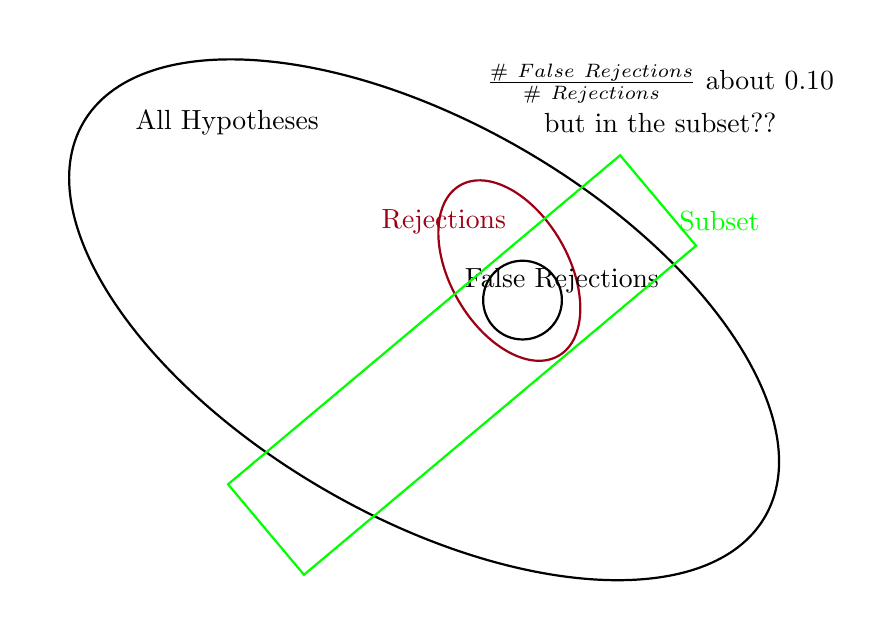
\begin{tikzpicture}[scale=2.5]
\draw[rotate=60,thick] (0,0) ellipse (1cm and 2cm);
\path (-1,1) node {All Hypotheses};
\draw[rotate=30,thick, redUnipd] (.5cm,0) ellipse (.3cm and .5cm);
\path[redUnipd] (.1,.5) node {Rejections};
\pause
\draw[rotate=00,thick, black] (.5cm,.1) ellipse (.2cm and .2cm);
\path[black] (.7,.2) node {False Rejections};
\path[black] (1.2,1.2) node {$\frac{\#\ False\ Rejections}{\#\ Rejections}$ about $0.10$};
\pause
\path[black] (1.2,1) node {but in the subset??};
\draw [rotate=40,green,thick] (-1.3, -.6) rectangle (1.3,0);
\path [green] (1.5,.5) node {Subset};
\end{tikzpicture}
\end{frame}




\bfr{Relationships between FWER and FDR}
  \bb{Dominance}
    \[ \mathrm{P}(V > 0) = \mathrm{E}(\boldsymbol{1}\{V > 0\}) \geq \mathrm{E}(\mathrm{FDP}) \]
    Consequence: Control of FWER implies control of FDR
  \eb
  \bb{Complete null hypothesis}
    If all hypotheses true, $\mathrm{FDP} = \boldsymbol{1}\{V > 0\}$
    \\ Consequence: If all hypotheses true, FDR $=$ FWER
  \eb
  \bb{Single hypothesis}
    If only one hypothesis, $\mathrm{FDP} = \boldsymbol{1}\{V > 0\}$
    \\ Consequence: If only one hypothesis, FDR $=$ FWER $=$ Type I error
  \eb
\end{frame}


\bfr{FWER vs.\ FDR: scaling}
  \bb{Scaling}
    As the size $m$ of the problem grows \\(complete null not true)
  \eb
  \bb{FWER}
    \bi
      \item Number of rejections remains limited
      \item Number of errors remains limited
    \ei
  \eb
  \bb{FDR}
    \bi
      \item Number of rejections grows with $m$
      \item Number of errors grows with $m$
    \ei
  \eb
\end{frame}


\bfr{When to use FDR}
%   \bb{Use FDR especially}
    \bi
      \item If collection of rejections important
      \item If validation experiments follow
      \item If hypotheses are exchangeable
      \item If power is an issue
    \ei
%   \eb
\end{frame}


\subsection{}
\bfr{Take-home message}
\bi 
\item Molteplicity control is mandatory in Clinical Trials 
\item FWER: controlling the probability of at least one error
\item FDR:  controlling the  proportion of false rejection (on average)
\item FWER is 
\bi
\item a stronger control
\item usually preferible in Clinical Trials
\item more flexible
\ei
\item FWER and FDR  easy in {\tt R}
\item excellent tutorial: Goeman \& Solari (2014) \footnote{
JJ Goeman, A Solari (2014) Tutorial in biostatistics: multiple hypothesis testing in genomics. Statistics in medicine, Volume 33, Issue 11}
\ei
\end{frame}



\end{document}


